\documentclass{beamer}

\mode<presentation>
{
  \usetheme{AnnArbor} %Copenhagen
  \usecolortheme{wolverine}
  \setbeamercovered{transparent}
}

\usepackage[english]{babel}
\usepackage[latin1]{inputenc}
\usepackage{times}
\usepackage[T1]{fontenc} 
% Or whatever. Note that the encoding and the font should match. If T1
% does not look nice, try deleting the line with the fontenc.
\usepackage{amsmath}
\usepackage{graphicx}

\newcommand{\linespace}{\vskip 0.25cm}

\definecolor{MyForestGreen}{rgb}{0,0.7,0} 
\newcommand{\tableemph}[1]{{#1}}
\newcommand{\tablewin}[1]{\tableemph{#1}}
\newcommand{\tablemid}[1]{\tableemph{#1}}
\newcommand{\tablelose}[1]{\tableemph{#1}}

\definecolor{MyLightGray}{rgb}{0.6,0.6,0.6}
\newcommand{\tabletie}[1]{\color{MyLightGray} {#1}}

% The text in square brackets is the short version of your title and will be used in the
% header/footer depending on your theme.
\title[Morphology in Art Restoration]{Morphological Operations Applied to \\ Digital Art Restoration}

% Sub-titles are optional - uncomment and edit the next line if you want one.
% \subtitle{Why does sub-tree crossover work?} 

% The text in square brackets is the short version of your name(s) and will be used in the
% header/footer depending on your theme.
\author[Dramdahl]{M. Kirbie Dramdahl}

% The text in square brackets is the short version of your institution and will be used in the
% header/footer depending on your theme.
\institute[U of Minn, Morris]
{
  Division of Science and Mathematics \\
  University of Minnesota, Morris \\
  Morris, Minnesota, USA
}

% The text in square brackets is the short version of the date if you need that.
\date[April '14, Sen. Sem., UMM] % (optional)
{29 April 2014 \\ UMM CSci Senior Seminar Conference \\ University of Minnesota, Morris}

% Delete this, if you do not want the table of contents to pop up at
% the beginning of each subsection:
\AtBeginSection[]
{
  \begin{frame}<beamer>
    \frametitle{Outline}
    \tableofcontents[currentsection, hideothersubsections]
  \end{frame}
}

\begin{document}

\begin{frame}
  \titlepage
\end{frame}

% For a 20-25 minute senior seminar talk you probably want something like:
% - Two or three major sections (other than the summary).
% - At *most* three subsections per section.
% - Talk about 30s to 2min per frame. So there should probably be between
%   15 and 30 frames, all told.

\section*{Overview}

\subsection*{Outline}

\begin{frame}
\frametitle{Why?}
Art restoration preserves objects of artistic, cultural, or historical value.
\linebreak
\linebreak
Digital art restoration provides:
\begin{itemize}
\item a comparatively inexpensive alternative.
\item a nondestructive tool.
\item an approximation of the initial appearance.
\end{itemize}
\end{frame}

\begin{frame}
  \frametitle{Outline}
  \tableofcontents[hideallsubsections]
\end{frame}

\section[Edge Detection]{Edge Detection}

\begin{frame}
\frametitle{Criteria}
\begin{enumerate}
\item Accuracy - low error rate
\linebreak
\item Localization - minimal distance between detected and actual edge
\linebreak
\item Uniqueness - only one response to a single edge
\end{enumerate}
\end{frame}

\begin{frame}
\frametitle{Canny Algorithm}
\begin{enumerate}
\item Smooth image by applying Gaussian filter.
\linebreak
\item Take gradient of image.
\linebreak
\item Identify regions containing significant jumps in intensity.
\linebreak
\item Search regions for local maximum.
\linebreak
\item Compare remaining pixels to two thresholds.
\end{enumerate}
\end{frame}

\section[Morphological Operations]{Morphological Operations}

\begin{frame}
\frametitle{Morphological Operations}
\begin{columns}
\begin{column}{0.5\textwidth}
Binary and Greyscale Images
\linebreak
\linebreak
Two Inputs:
\begin{itemize}
\item Original Image
\item Structuring Element
\end{itemize}
\end{column}
\begin{column}{0.5\textwidth}

\includegraphics[width=1\textwidth,trim={0 6.5in 4in 0},clip]{structuring_element_placement}
\end{column}
\end{columns}
\end{frame}

\subsection[Erosion]{Erosion}

\begin{frame}
\frametitle{Erosion}
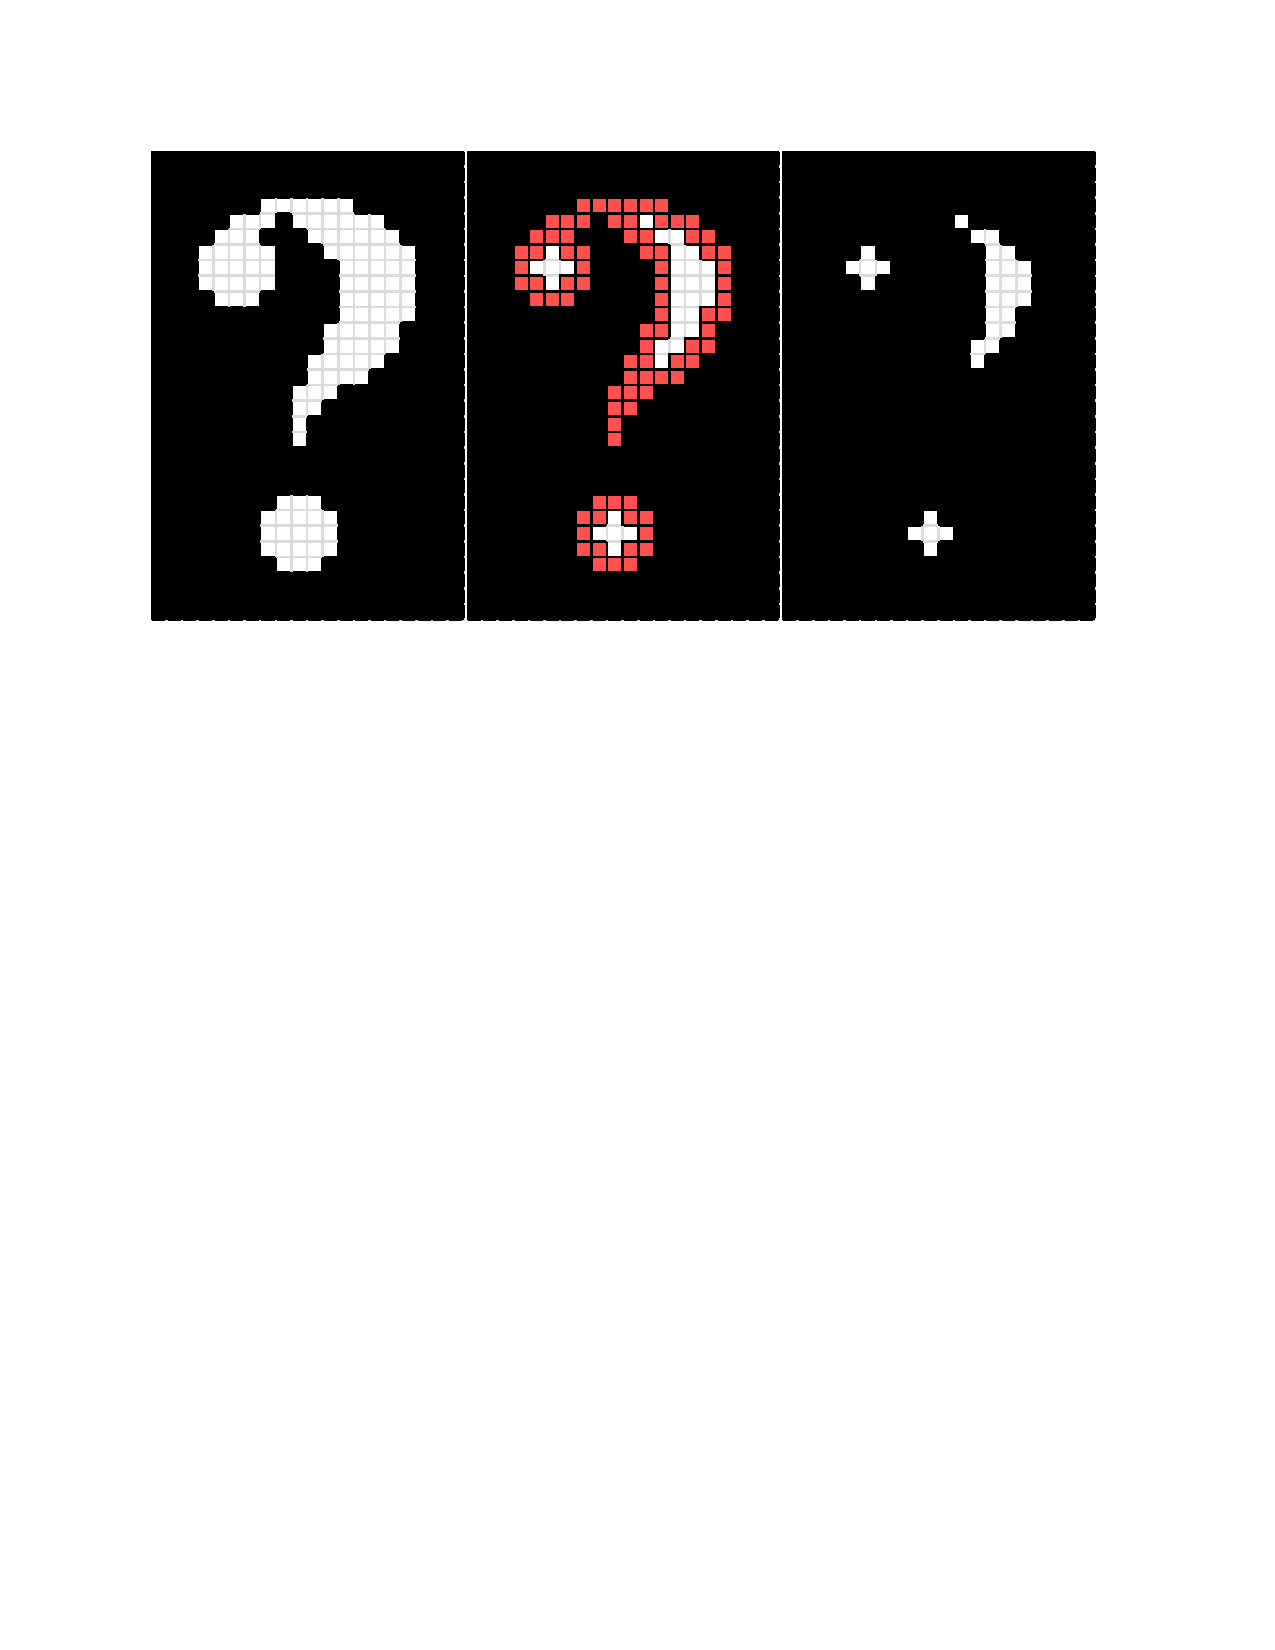
\includegraphics[width=1\textwidth]{erosion}
\end{frame}

\subsection[Dilation]{Dilation}

\begin{frame}
\frametitle{Dilation}

\includegraphics[width=1\textwidth]{dilation}
\end{frame}

\subsection[Opening]{Opening}

\begin{frame}
\frametitle{Opening}
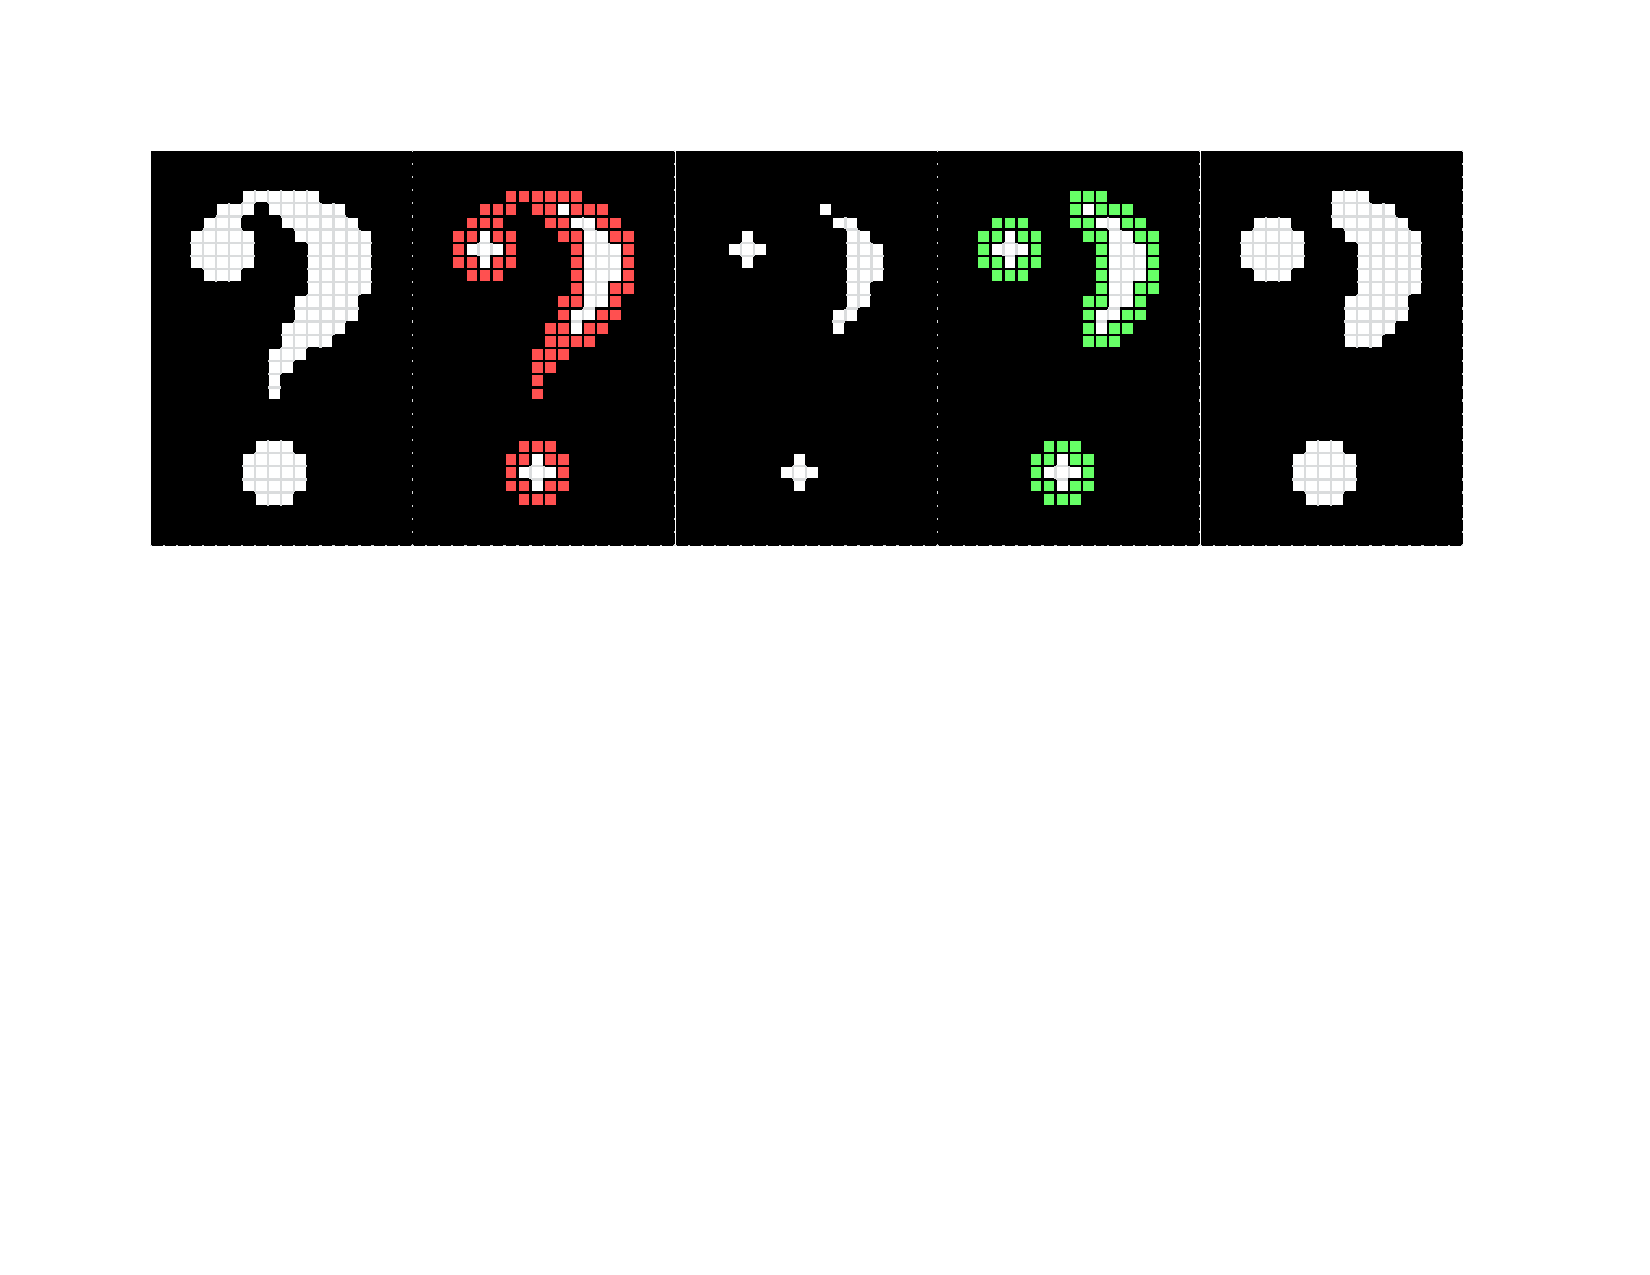
\includegraphics[width=1\textwidth]{opening}
\end{frame}

\subsection[Closing]{Closing}

\begin{frame}
\frametitle{Closing}

\includegraphics[width=1\textwidth]{closing}
\end{frame}

\section[Methods of Crack Detection]{Methods of Crack Detection}

\subsection[Top-Hat Transform]{Top-Hat Transform}

\begin{frame}
\frametitle{Top-Hat Algorithm}
Three Variations:
\begin{itemize}
\item Black Top-Hat
\item White Top-Hat
\item Multiscale Top-Hat
\end{itemize}
\end{frame}

\subsubsection[Black Top-Hat]{Black Top-Hat}

\begin{frame}
\frametitle{Black Top-Hat Transform}
Darker Details on a Lighter Background
\linebreak
\linebreak
$BTH = (f \bullet s) - f$
\end{frame}

\subsubsection[White Top-Hat]{White Top-Hat}

\begin{frame}
\frametitle{White Top-Hat Transform}
Lighter Details on a Darker Background
\linebreak
\linebreak
$WTH = f - (f \circ s)$
\end{frame}

\subsubsection[Multiscale Top-Hat]{Multiscale Top-Hat}

\subsection[Alternative Method]{Alternative Method}

\section[Inpainting]{Inpainting}

\begin{frame}
\frametitle{Inpainting Process}
The image is broken down into regions, which are further broken down into neighborhoods. For each defective pixel $i$:
\begin{enumerate}
\item Find the context of $i$.
\item Examine all other neighborhoods within the region of $i$.
\item Find neighborhood most similar to context of $i$ by sum of squared differences.
\item If the sum of squared errors is below a set threshold, replace all defective pixels in the neighborhood of $i$ with corresponding pixels from most similar neighborhood.
\item Otherwise, replace pixel $i$ with the median value of all non-defective pixels within its neighborhood.
\end{enumerate}
\end{frame}

\section[Results]{Results}

\subsection[Top-Hat Transform Results]{Top-Hat Transform Results}

\subsection[Alternative Method Results]{Alternative Method Results}

\section[Conclusions]{Conclusions}

\begin{frame}
	\frametitle{Thanks!}
		
	\linespace
	\linespace
	
	%Contact: \texttt{dramd002@morris.umn.edu}
	
	\linespace
	\linespace
	
	\begin{center}
	{\huge Questions?}
	\end{center}
\end{frame}

\section*{References}

\begin{frame} 
	\frametitle{References} 
	
	\begin{thebibliography}{lskdjf}
	\end{thebibliography}
\end{frame} 

\end{document}